\documentclass{sig-alternate}
% \documentclass{acm_proc_article-sp}
\usepackage{graphicx}
\usepackage{hyperref}

\usepackage{subfig}
%\usepackage{caption}
\DeclareCaptionType{copyrightbox}
%\usepackage{subcaption}

\usepackage{verbatim}
\makeatletter
\newif\if@restonecol
\makeatother
\let\algorithm\relax
\let\endalgorithm\relax
\usepackage[linesnumbered]{algorithm2e}

\makeatletter
\newcommand{\nosemic}{\renewcommand{\@endalgocfline}{\relax}}% Drop semi-colon ;
\newcommand{\dosemic}{\renewcommand{\@endalgocfline}{\algocf@endline}}% Reinstate semi-colon ;
\newcommand{\pushline}{\Indp}% Indent
\newcommand{\popline}{\Indm\dosemic}% Undent
\makeatother

\pdfinfo{
   /Title  (acm-mm13-short)
}

\begin{document}

\title{Generating Infographics with Context Discovery Principles}

\numberofauthors{2}
\author{
\alignauthor
Person 1\\
       \affaddr{University}\\
       \email{email}\\
\alignauthor
Person 2\\
       \affaddr{University}\\
       \email{email}\\
}


\maketitle
\begin{abstract}
Something abstract.
\end{abstract}

\category{H.3.3}{Information Search and Retrieval}{Information Filtering}
\category{H.3.4}{Systems and Software}{Information Networks}
\category{H.5.1}{Multimedia Information Systems}{} 

\terms{Design, Algorithms, Experimentation}
\keywords{CueNet, context, discovery, event, personal, photo, tagging}

\section{Introduction}
Intro

\section{Context}
Some context about context.

\section{Progressive Discovery}
Blah \cite{westermann2007toward, gupta2011managing}



\begin{figure}[t]
\centering
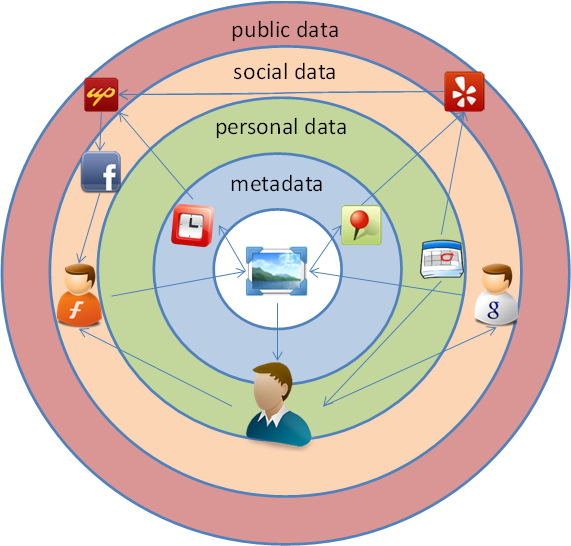
\includegraphics[width=0.48\textwidth]{media/prog-discovery.png}
\caption{Example of Progressive Discover.}
\label{fig:cuenet-arch}
\end{figure}

\bibliographystyle{abbrv}
\bibliography{sigproc}
\end{document}
